\chapter{Results and Discussion}\label{results}
%All our results are in ones and zeroes. 
%And further we discuss why there are only zeroes. And how that affects the
%outcome and future endeavors for the pirates we are. 

The results of our research and the following discussion of them happen here.
We touch the main parts of the thesis. The data sources, section
\ref{results:data_sources}. Dictionaries, section \ref{results:dictionaries}. Classification of sentiment in section
\ref{results:classification}. And the trend in section \ref{results:trend}.
Last we have a general discussion about the results. 
%

\section{Data Source}\label{results:data_sources}
Twitter as a data source proved to be OK. It was quite easy to obtain data. But
increasingly difficult to get good amounts of data and unbiased data. All the
initial data have some restriction to search words or other limits. In total we
should have mined a lot more data and manually classified more of it. 

As far as the dictionaries go they work well. We have different results for
different dictionaries and different datasets, but all in all the way to
compile datasets work good. The dictionaries depend on the manually classified
tweets, so a lot of the potential improvement lies there. Although we can
improve the dictionaries by removing stop words and other words we know have no
clear positive of negative sentiment. 

In research question 1, \ref{introduction:rq1}, we asked what knowledge we can
extract from tweets to find a sentiment. The dictionaries are a good way to
compose sentiment from the different words in the manually labeled tweets.

Research question 3, \ref{introduction:rq3}, asks if Twitter has been useful in
comparison with technical analysis. To some  extent it has. We have mined and
classified many tweets in the hope that the aggregated trend would show
likeness to plots of technical analysis. The data from Twitter that has been
used to acquire positive and negative tweets for the trend aggregation. And has
also provided useful insight into the use of the Twitter API. 
%

\section{Dictionaries}\label{results:dictionaries}
As for the use of the dictionaries in association with the trend and research
question 3, \ref{introduction:rq3}, we use the dictionaries for feature
extraction in the classifiers. Besides the use in classifiers the dictionaries
have no other practical uses in this thesis in relation to sentiment.

\paragraph{Error analysis}
\hspace{0pt}\\
When looking at the duplicate words from the monogram dictionary based on the
kiro dataset we found some errors.
As a selection of words found, we have \textit{dangerous, bad, go, inc, let, up,
or, need, good, if, no, are, and, of, on, the,
is, as}.
Here we can see that the words \textit{good} and \textit{bad} are represented.
Which is not good. By removing the words from the dictionaries we have removed
significant words in further classification, thus reducing correctness of the
algorithm. This is one of the drawbacks of the monogram dictionaries.

When looking at the removed duplicate words for bigram and trigrams we found no
indication of the same problem. As the uniqueness of bigrams and trigrams are a
lot greater we end up with very few duplicates and only duplicates that has no
significance to the over all classification. Although we might have other
unknown problems.

Most stop words and other insignificant words are removed with the removal of
duplicate words. The same thing cannot be said about the bigram and trigram
dictionaries. There we have no stop words present in themselves, but they are
frequently part of other terms. For further improvements of classification with
word counting and dictionary quality we should remove
stop words, such as \textit{as, is, on, off, and, or} etc, from the
tweet/sentence before creating bi- and trigrams.
%

\section{Classification}\label{results:classification}
Manual labeling is a bit of a challenge to keep unbiased. The whole
classification process is based on a persons opinion, which makes the results
somewhat biased. To eliminate this error we should have multiple people do the
manual classification and combine the results.  

Word counting works to some extent. But presents varied results based on the
dataset and the dictionary used. Again this comes down to the dataset and the
dictionaries created. Also the way we separate tweets from each other with a
threshold can be improved. All in all word counting works, but it is not very
good. 

Classifiers  improve the classification quite a bit. With the svm classifier we
get around 98 percent correct classification on both data sets. Which is good.

The uncertainties lie in the biased, or potentially biased, data. We do not
know if the data in itself is fully representable for the content on twitter.
Neither do we know if the manual classification is completely correct. 

In total we gained some knowledge about dictionaries and their effect on
classification. And we can confirm that classifiers work better than word
counting.  

We tested two ways of finding the sentiment of a tweet. The bag of words method
described in section \ref{sentiment:word_count_classification}, and the
classifier way with the SVM and Naive Bayes classifiers,
\ref{sentiment:classification}.

Research question 2, \ref{introduction:rq2}, the question of trend aggregation,
the classification was useful. The sentiment worked to some extent. We do not
know how well. And we have to look into the part of credibility in future work.   
%

\subsection{Word Count Classification}\label{results:word_count_classification}
The results from the word count classification can be plotted in the tabled
\ref{tbl:sentiment_word_count_results} and in the graph
\ref{tbl:sentiment_word_count_results}.

\begin{table}
\centering
\label{tbl:sentiment_word_count_results}
\caption{Word Count classification results table}
\begin{tabular}{ r p{6cm} r r c }
id & Dictionary & Failed & Correct & Accuracy \\
& -- Kiro compiled dataset -- & a & b & b/(a+b) \\
\hline
1 & Monogram, obama & 578 & 419 & 0.4203 \\
2 & Monogram LoughranMcDonald & 491 & 506 & 0.5075 \\
3 & Monogram, combined Obama and LoughranMcDonald & 416 & 581 & 0.5827 \\
4 & Kiro, Monogram, self compiled & 115 & 882 & 0.8847 \\
5 & Kiro, Bigram, self compiled & 17 & 980 & 0.9829 \\
6 & Kiro, Trigram, self compiled & 18 & 979 & 0.9819 \\
7 & Obama, Monogram, self compiled & 567 & 430 & 0.4313 \\
8 & Obama Bigram, self compiled & 534 & 463 & 0.4644 \\
9 & Obama Trigram, self compiled & 567 & 430 & 0.4313 \\
& -- Obama tweet set -- & a & b & b/(a+b) \\
\hline
10 & Monogram, obama & 855 & 510 & 0.3736 \\
11 & Monogram LoughranMcDonald & 508 & 857 & 0.6278 \\
12 & Monogram, combined Obama and LoughranMcDonald & 544 & 821 & 0.6015 \\
13 & Kiro, Monogram, self compiled & 632 & 733 & 0.5370 \\
14 & Kiro, Bigram, self compiled & 521 & 844 & 0.6183 \\
15 & Kiro, Trigram, self compiled & 498 & 867 & 0.6352 \\
16 & Obama, Monogram, self compiled & 493 & 872 & 0.6388 \\
17 & Obama Bigram, self compiled & 37 & 1328 & 0.9729 \\
18 & Obama Trigram, self compiled & 39 & 1326 & 0.9714 \\
\end{tabular}
\end{table}

5, 6, 17, 18 are the dictionaries with best accuracy. Which is to be expected
for the classification of the dataset the dictionary was created from.

But more interestingly, if we take the dictionaries created form one dataset,
and look at the results of the classification on the other dataset. We compare
7, 8, 9 with each other and 13, 14, 15 with each other. Then we can see that
the bigram and trigram dictionaries perform overall better than the monogram
dictionaries.

Further we see indications that the quality of the dictionary plays an
important role. The LoguhranMcDonald monogram dictionary performs quite good
with both datasets. Even on par with the compiled dictionaries on opposite
dataset. This indicates that a well crafted dictionary can perform as well
as compiled dictionaries.

\begin{figure}[htb]
    \centering
    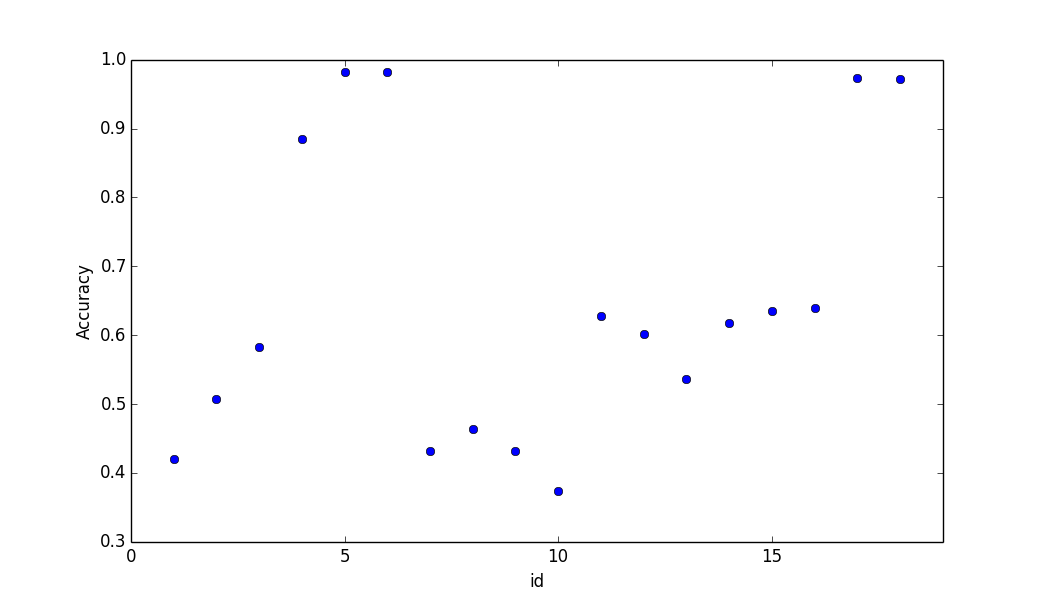
\includegraphics[width=\textwidth]{dictionary_accyracy.png}
    \label{fig:dictionary_accyracy}
    \caption{Dictionary Accuracy plot}
The graph shows the plotted accuracies from the word count
classification. The ids represents the ids from the table above,
\ref{tbl:sentiment_word_count_results}
\end{figure}

When comparing the results from one dataset to the other we can see indications
of how the content of the dataset also plays a huge role in the results. Some
tweets are more difficult to classify then others.

There are a lot of improvements that could be done.
The word count classification is merely a convenient way to say something about
the dictionaries used. We should expand our knowledge toward the quality of the
dictionaries. And look for ways to eliminate terms that are neither positive or
negative. 

\subsection{Threshold Variation}\label{results:threshold}
Further we found the best average threshold value to be 0.1.
From the table under we have the threshold value, and the average
classification accuracy among the 18 entries for each threshold value.

\begin{table}
\centering
\label{tbl:average_threshold_accuracy}
\caption{Average threshold accuracy table.}
\begin{tabular}{ c c c c }
Threshold & Accuracy & Threshold & Accuracy \\
\hline
- & - & 0.0 & 0.6479 \\
-0.1 & 0.6316 & 0.1 & 0.6516 \\
-0.2 & 0.6161 & 0.2 & 0.6511 \\
-0.3 & 0.6059 & 0.3 & 0.6430 \\
-0.4 & 0.5988 & 0.4 & 0.6305 \\
-0.5 & 0.5888 & 0.5 & 0.6122 \\
-0.6 & 0.5711 & 0.6 & 0.5934 \\
-0.7 & 0.5423 & 0.7 & 0.5712 \\
-0.8 & 0.5083 & 0.8 & 0.5457 \\
-0.9 & 0.4881 & 0.9 & 0.5307 \\
\end{tabular}
\end{table}

\begin{figure}[htb]
    \centering
    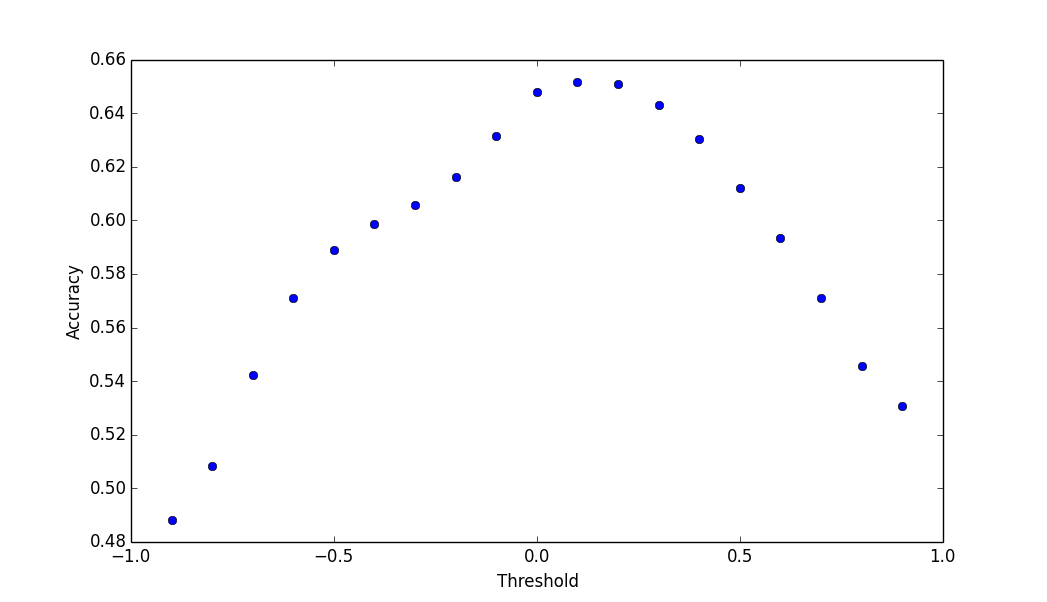
\includegraphics[width=\textwidth]{average_threshold_accuracy.png}
    \label{fig:average_threshold_accuracy}
    \caption{Average threshold accuracy}
Graph plots of the 'Average threshold accuracy' table.
\end{figure}

In figure \ref{fig:threshold_graphs} we list the results of the experimentation
with the threshold. Table \ref{tbl:dictionary_to_threshold} lists the
dictionaries and dataset used for which graphs in figure
\ref{fig:threshold_graphs}.
'kiro dataset' and 'obama dataset' columns tells which dataset that was
classified in which graph.

\begin{table}
\centering
\label{tbl:dictionary_to_threshold}
\caption{Dictionary to threshold graph plot table}
\begin{tabular}{ l c c }
Dictionary name and description & kiro dataset & obama dataset \\
\hline
Obama original, Monogram & 1 & 10 \\
LoughranMcDonald, Monogram & 2 & 11 \\
Combined Obama original and \\ LoughranMcDonald, Monogram & 3 & 12 \\
Kiro, Monogram, self compiled & 4 & 13 \\
Obama, Monogram, self compiled & 5 & 14 \\
Kiro, Bigram, self compiled & 6 & 15 \\
Obama, Bigram, self compiled & 7 & 16 \\
Kiro, Trigram, self compiled & 8 & 17 \\
Obama, Trigram, self compiled & 9 & 18 \\
\end{tabular}
\end{table}

\begin{figure}[htb]
    \centering
    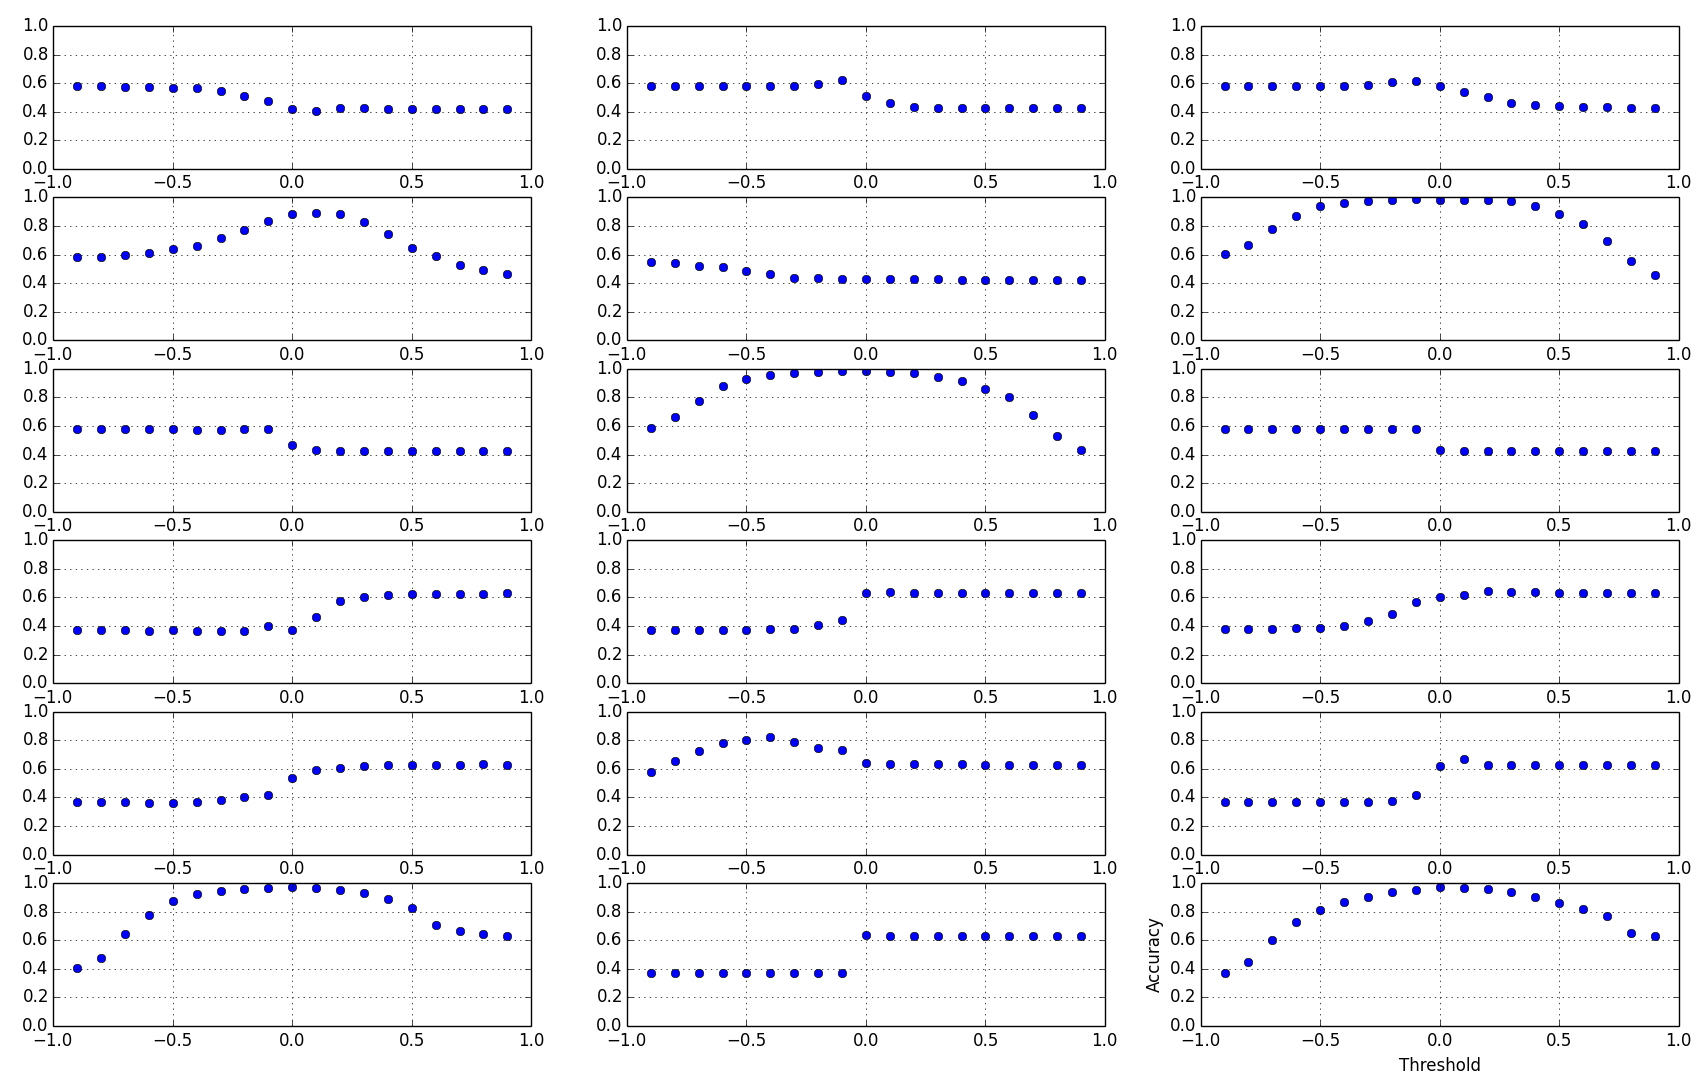
\includegraphics[width=\textwidth]{threshold_graphs.png}
    \label{fig:threshold_graphs}
    \caption{Threshold variation accuracy plot}
The graphs plot the different variations of threshold. Counting is
columns first; top left is 1, top mid is 7, top right is 13.
\end{figure}

\subsection{Using Classifiers}
Not surprisingly the classifiers have better results than the bag of words
method of classification. Further the SVM classifier with the LinearSVC kernel
module performed best. Naive Bayes classifier was nearly as good. This answers
part of research question 1, \ref{introduction:rq1}.

\paragraph{SVM}\label{results:svm_classification}
\hspace{0pt}\\
From results of the experiment, \ref{experiments:svm_classification}, we can draw
some conclusions. The monogram dictionary performed
better than the bigram dictionary. Probably due to the number of features we
can extract from each tweet. Also classifiers are more accurate than the word
count classification method.

\paragraph{Naive Bayes}\label{results:naive_bayes_classification}
\hspace{0pt}\\
As we can see from the experiment,
\ref{experiments:naive_bayes_classification}, the different dictionaries makes
no difference for the Naive Bayes classifier. But if we compare the classifier
with the results from the word count classification we can clearly see
improvement. 

\subsection{Comparison}\label{results:comparison}
In the following table, \ref{tbl:classification_comparison}, we highlight the
results from the different classifications. We list the most noteworthy results
from our experiments and compare them.

\begin{table}
\centering
\label{tbl:classification_comparison}
\caption{Comparison of classifiers table}
\begin{tabular}{ l l p{3.5cm} r r c }
Classifier & Dataset & Dictionary & Failed & Correct & Accuracy \\
\hline
Word Count & Kiro & Obama Bigram & 534 & 463 & 0.4644 \\
Word Count & Obama & LoughranMcDonald Monogram & 508 & 857 & 0.6278 \\
Word Count & Obama & Kiro, Trigram & 498 & 867 & 0.6352 \\
Naive Bayes & Kiro & Kiro Monogram & 29 & 968 & 0.9709 \\
SVM & Kiro & Kiro Monogram & 7 & 990 & 0.9930 \\
\end{tabular}
\end{table}

As we can see the classifiers give better results then the word count
classification. And SVM is a bit better than Naive Bayes. Although the results
from the word count classification indicates that the dictionaries play an
important role in the results. We can also see that monograms are better for
classifiers, while trigrams are better for word counting.

For the classifiers and the good results with the monogram dictionaries, we
think
that has to do with the number of features we get from a tweet. The more
features we have the easier it is to classify and the more accurate the result.
%

\section{The Trend}\label{results:trend}
Comparing the two graph plots, figure \ref{fig:trend_finance_plot} and figure
\ref{fig:trend_tweet_plot}, we can see minor similarities. All the moving
averages have rightward growth. While for the tweet trend the 3 day interval
preforms worse than the 8 day interval. There are no certain correlations
between the two trends. And it is difficult to conclude on specifics. 

For the research questions, 2(\ref{introduction:rq2}), and
3(\ref{introduction:rq3}) are in some degree true. RQ2, we can aggregate a
trend. But the use for it and the accuracy we know nothing of. RQ3 has the
answer poor. The sentiment trend compares poorly to the trend from the technical
analysis. 
%

\section{Discussion}\label{results:discussion}
From the three parts we have satisfying and unsatisfying results. We have good
results and vague results. The vague results should be frowned upon. While the
reasonable results should be expanded, retested and improved. 
Most notably we have clear indications that dictionaries, automatically compiled
from a manually classified tweets set, can be used when classifying sentiment. 

The accomplished research, based on the research questions(RQ), can be described as
satisfactory. We set out to investigate how we can determine then sentiment of
a tweet, \ref{introduction:rq1}, how Twitter can be used to aggregate a trend,
\ref{introduction:rq2}, and hod Twitter based trends compare the technical
analysis in stock markets, \ref{introduction:rq3}. 

RQ1 more specifically aims at the information of tweets, the knowledge we
can extract from them and classification of sentiment. In all respects we
gained new knowledge. By creating dictionaries we extracted words from
manually labeled tweets, giving us a way to classify new tweets. We ended up
only using the tweet text for classification. Other metadata should have been
explored. The best way of classifying tweets we found to be the SVM classifier.    
RQ2 reaches the complicated part of aggregating a trend based on Twitter. This
turned out to be difficult. Mainly by the lack of good ideas of how we could do
it, but also the difficulty of transforming data to a usable format. In the end
we transformed tweet data to the same format as stock data and used that for
the trend aggregation. 

RQ3 takes the trend a step further and compares technical analysis with the
Twitter based trend. After plotting moving average and average directional
index for both finance and Twitter data we compared the graphs. The two plots
can be seen in figure \ref{fig:trend_finance_plot}, and figure
\ref{fig:trend_finance_plot}. In the figures we looked for similarities. 
First the ADX, we have no similarities between the Twitter trend and the
finance trend. For the moving average(MA) we can argue that the blue lines, MA
with 8 day intervals, are quite similar. Although we can make no definite
conclusion that the Twitter trend is representative for the finance market.
Technical analysis is still better, but sentiment is a possibility. 
%
